% !TeX root = main.tex

% ============================================================
% thesis-sync entry: 2026-07-19_inchworm-pneumatic-system-circuit
% Type: design decision + numeric data (pneumatic architecture + control PCB)
% Part of the INCHWORM ROBOT block (prior work, precedes the lizard sections).
% Insertable section block (no preamble). Requires: graphicx, multirow, makecell.
%
% FIGURES STILL MISSING (author to drop files into figures/ then uncomment):
%   figures/pneumaticSchematic.png  (KiCad schematic export)   -> Fig circuit
%   figures/electronicsRender.png   (KiCad 3D render)          -> Fig render
%   figures/inflation.png figures/deflation.png figures/holding.png -> Fig states
% figures/pneumaticSystemFull.eps IS staged (assumed = full-system photo; CONFIRM).
%
% WIRING TABLES built from the exported KiCad netlist. Certain from the netlist:
% Arduino GPIO -> ULN2803A inputs, and ADS1115 I2C addressing. The driver-output
% -> valve-connector order and the sensor-channel order follow the board layout
% (footnoted). See the .md for the full list of flagged schematic simplifications.
% ============================================================

\section{PNEUMATIC CONTROL SYSTEM AND CIRCUIT DESIGN}
\label{sec:inchworm-pneumatics}

\subsection{Pneumatic Architecture}

The architectural design of the soft robot, incorporating three internal
actuation chambers and two distal suction cups, mandates a pneumatic control
system featuring a minimum of five independent pressure channels to ensure
operation of each functional unit. Moreover, the system must supply both
positive and negative gauge pressures, to respectively inflate the actuator
chambers and generate the vacuum for the suction cups. Inspired by the
architecture proposed by Xiao et al.~\cite{Xiao2023Programmable}, a custom
programmable pneumatic system was developed, featuring eight independent
channels driven by a shared positive-pressure pump and a shared vacuum pump
(DP0110T-Y1, Nitto Kohki). The system is governed by a microcontroller
(Arduino Mega 2560) that dictates the state of two normally closed solenoid
valves (2V025-08, RIH) per channel, enabling discrete inflation, deflation,
and holding states. Closed-loop pressure control is enabled by pressure
sensors (XGZP6847A100KPGPN, CFSensors) integrated into each output channel.

The three valve states are illustrated in Fig.~\ref{fig:inchworm-states}.
During inflation, the positive pump is activated and the corresponding
inflation valve opens while the exhaust valve remains isolated. Deflation is
achieved symmetrically by engaging the vacuum pump and opening the exhaust
valve. Once the measured pressure in a given channel reaches the desired
target within a tolerance of $\pm 1$~kPa, both valves are sealed to hold the
current state.

\begin{figure}[tb]
  \centering
  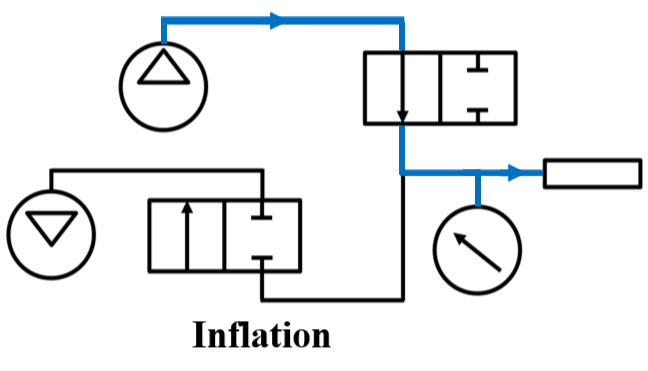
\includegraphics[height=26mm]{figures/inflation.png}\hfill
  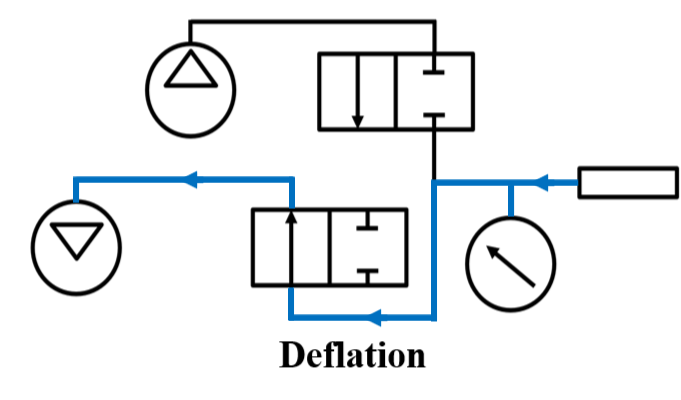
\includegraphics[height=26mm]{figures/deflation.png}\hfill
  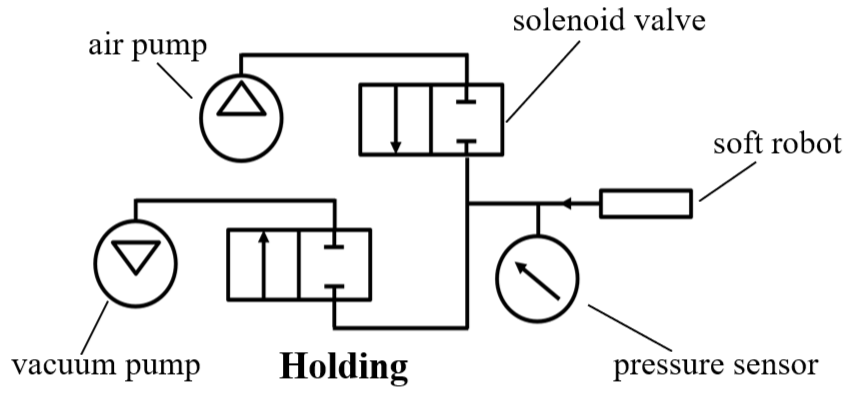
\includegraphics[height=26mm]{figures/holding.png}
  \vspace*{-1mm}
  \caption{The three per-channel valve states of the pneumatic system.
  (Left) Inflation: the positive (air) pump is engaged and the inflation
  solenoid valve opens while the exhaust valve stays closed, admitting air
  to the soft robot. (Center) Deflation: the vacuum pump is engaged and the
  exhaust valve opens while the inflation valve stays closed, drawing air
  out. (Right) Holding: both solenoid valves are sealed and the channel
  pressure, monitored by the in-line pressure sensor, is maintained.}
  \label{fig:inchworm-states}
\end{figure}

\begin{figure}[tb]
  \centering
  \includegraphics[width=0.9\columnwidth]{figures/pneumaticSystemFull.eps}
  \vspace*{-1mm}
  \caption{The assembled eight-channel pneumatic control box, housing the
  shared positive and vacuum pumps (DP0110T-Y1, Nitto Kohki), the sixteen
  solenoid valves (2V025-08, RIH) on their manifolds, the 12~V switching
  power supply, the step-down and boost converters for the logic and pump
  rails, and the Arduino Mega 2560 carrying the custom driver shield.}
  \label{fig:inchworm-systemphoto}
\end{figure}

\subsection{Control Electronics}

The control electronics were consolidated onto a custom shield mounted
directly on the Arduino Mega 2560, whose layout was first validated in a
KiCad design (Fig.~\ref{fig:inchworm-render}) before assembly. The complete
schematic is shown in Fig.~\ref{fig:inchworm-schematic}. For legibility, the
per-channel sensing and actuation wiring is drawn explicitly for a
representative subset of the channels and replicated identically for the
remaining ones; the physical system implements all eight channels.

Each of the sixteen solenoid valves is switched on the low side by one
channel of a ULN2803A Darlington-array driver, two such arrays providing the
sixteen channels. The valve coils are commoned to the 12~V rail through each
driver's COM pin, which returns the coil fly-back current. The
Arduino-pin-to-valve assignment used by the firmware is listed in
Table~\ref{tab:inchworm-valvewiring}: the preliminary schematic routed the
valve inputs through pins $D22$--$D37$, but these were reassigned during the
hand-assembly of the perfboard shield, and the firmware mapping reflects the
as-built wiring. The eight pressure sensors are read over a single
$\mathrm{I^2C}$ bus ($SDA=D20$, $SCL=D21$) by two ADS1115 16-bit
analog-to-digital converters, addressed at $\mathtt{0x48}$ and
$\mathtt{0x49}$ (four sensor channels each). The two shared pumps are
switched by logic-level N-MOSFETs (IRLZ44N) commanded by pins $D13$
(positive pump) and $D12$ (vacuum pump), each with a 1N4007 fly-back diode
across the pump; two 0.5~F bulk capacitors buffer the current surges drawn by
the pumps and valve coils.

The system draws power from a 12~V, 10~A switching supply (S-120-12). This
12~V rail directly feeds the sixteen solenoid valves; a boost converter
derives the 24~V rail that drives the two shared pumps, and a step-down
converter derives the 5~V logic rail that powers the Arduino, the ADS1115
modules, and the pressure sensors. In the schematic these rails are drawn in
a simplified manner: the logic and sensor supplies share the ``$+12$V'' net
label although they are physically at 5~V, and the ``$+24$V'' annotation at
the pump stage denotes the boost-converter output, which is not itself drawn
as a discrete component.

\begin{figure}[tb]
  \centering
  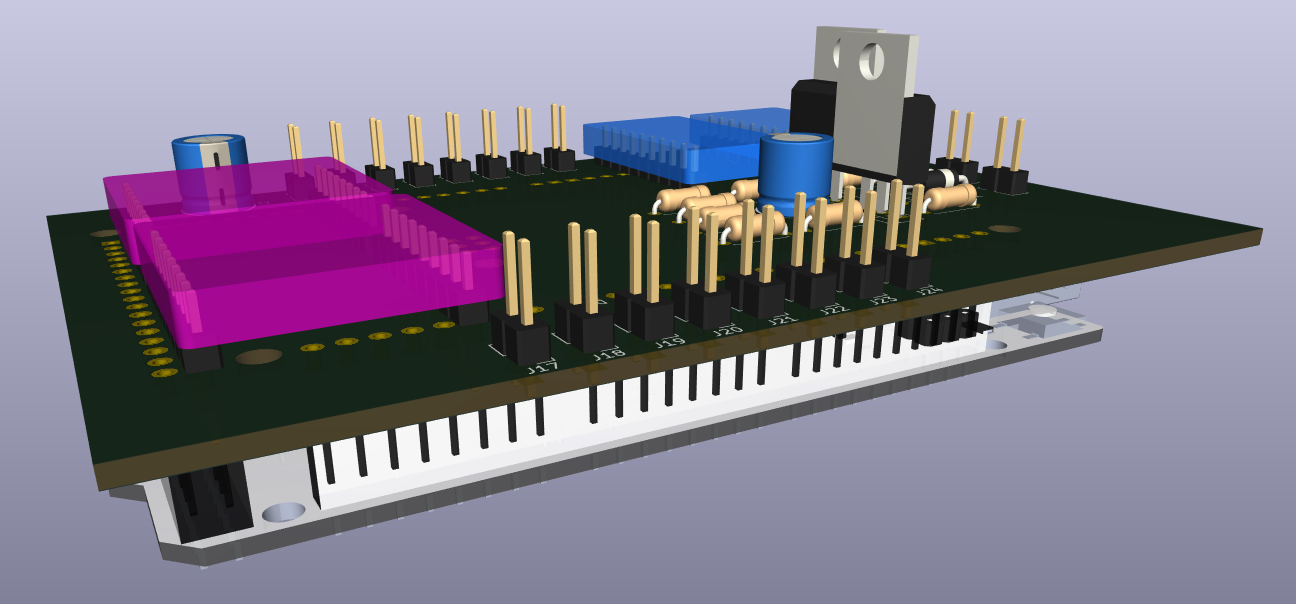
\includegraphics[width=0.95\columnwidth]{figures/electronicsRender.png}
  \vspace*{-1mm}
  \caption{Compact layout of the Arduino Mega driver shield, rendered in
  KiCad prior to fabrication. The board carries the two ULN2803A valve
  drivers, the ADS1115 sensing modules, the pump MOSFET stage, and the
  screw-terminal connectors for the valves, sensors, and pumps.}
  \label{fig:inchworm-render}
\end{figure}

\begin{figure*}[tb]
  \centering
  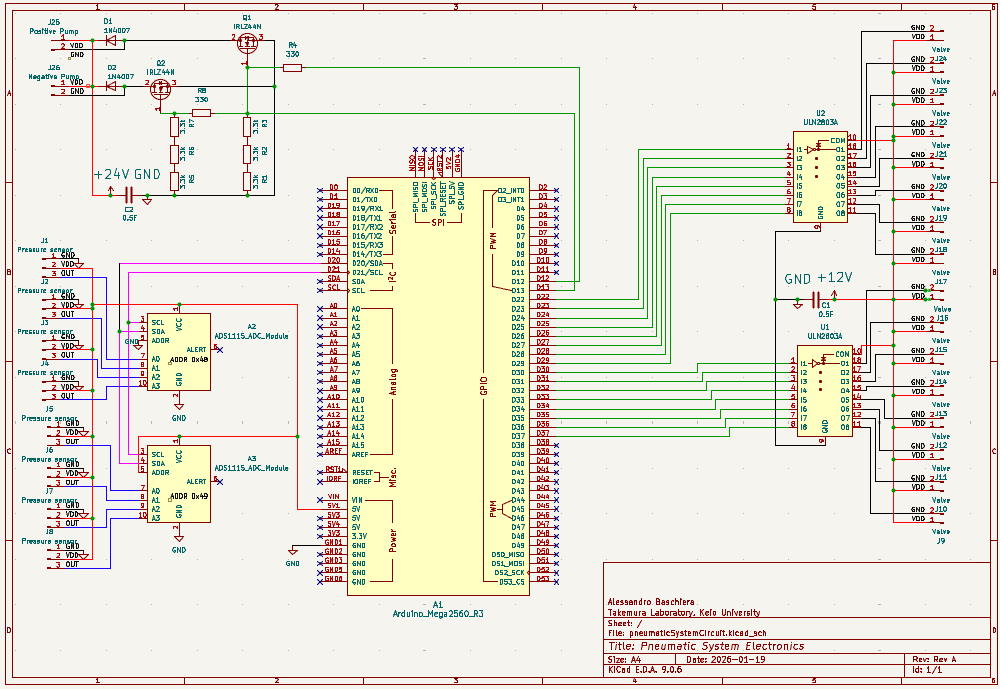
\includegraphics[width=0.95\textwidth]{figures/pneumaticSchematics.png}
  \vspace*{-1mm}
  \caption{Schematic of the eight-channel pneumatic control electronics
  (KiCad). The Arduino Mega 2560 shield drives sixteen solenoid valves
  through two ULN2803A Darlington arrays and acquires the eight channel
  pressures through two ADS1115 converters over $\mathrm{I^2C}$; the two
  shared pumps are switched by IRLZ44N MOSFETs. For clarity the schematic
  details a representative subset of channels, with the remainder drawn as
  identical replicas.}
  \label{fig:inchworm-schematic}
\end{figure*}

\subsection{Wiring}

Table~\ref{tab:inchworm-bom} summarizes the electronic components, and
Tables~\ref{tab:inchworm-valvewiring} and~\ref{tab:inchworm-sensorwiring}
give the valve-actuation and pressure-sensing wiring, respectively. The
sixteen solenoid valves are grouped by the firmware into eight
(inflation, exhaust) pairs, one pair per pneumatic channel.

\begin{table}[tb]
  \caption{Bill of materials of the pneumatic control electronics.}
  \label{tab:inchworm-bom}
  \centering
  \footnotesize
  \setlength{\tabcolsep}{4pt}
  \begin{tabular}{|c|l|l|}
    \hline
    Ref. & Component & Function \\ \hline
    $A1$ & Arduino Mega 2560 R3 & Main controller \\ \hline
    $U1,U2$ & ULN2803A & 8-ch Darlington valve driver \\ \hline
    $A2,A3$ & ADS1115 & 16-bit $\mathrm{I^2C}$ ADC (4~ch each) \\ \hline
    $Q1,Q2$ & IRLZ44N & Logic-level N-MOSFET (pump switch) \\ \hline
    $D1,D2$ & 1N4007 & Pump fly-back diode \\ \hline
    $C1,C2$ & 0.5~F & Rail bulk/buffer capacitor \\ \hline
    $R4,R8$ & 330~$\Omega$ & MOSFET gate series resistor \\ \hline
    \makecell[l]{$R1$--$R3$,\\$R5$--$R7$} & 3.3~k$\Omega$ & MOSFET gate bias/pull-down \\ \hline
    $J1$--$J8$ & \makecell[l]{Pressure sensor\\(XGZP6847A100KPGPN)} & Channel pressure feedback \\ \hline
    $J9$--$J24$ & Valve (2V025-08) & Solenoid valve connectors \\ \hline
    $J25,J26$ & \makecell[l]{Pump (DP0110T-Y1)} & Positive / vacuum pump \\ \hline
  \end{tabular}
\end{table}

\begin{table}[tb]
  \caption{Valve and pump control mapping, as defined in firmware. Each
  pneumatic channel has one inflation and one exhaust solenoid valve, each
  switched (low side) through a ULN2803A Darlington channel; the two shared
  pumps are switched by the IRLZ44N MOSFETs.}
  \label{tab:inchworm-valvewiring}
  \centering
  \footnotesize
  \setlength{\tabcolsep}{6pt}
  \begin{tabular}{|c|c|c|}
    \hline
    Channel & \makecell{Inflation valve\\(Arduino pin)} & \makecell{Exhaust valve\\(Arduino pin)} \\ \hline
    1 & $D42$ & $D36$ \\ \hline
    2 & $D44$ & $D34$ \\ \hline
    3 & $D46$ & $D32$ \\ \hline
    4 & $D48$ & $D30$ \\ \hline
    5 & $D50$ & $D28$ \\ \hline
    6 & $D52$ & $D26$ \\ \hline
    7 & $D51$ & $D24$ \\ \hline
    8 & $D53$ & $D22$ \\ \hline
    \multicolumn{3}{|c|}{Shared positive pump: $D13$ \quad\quad Shared vacuum pump: $D12$} \\ \hline
  \end{tabular}
\end{table}

\begin{table}[tb]
  \caption{Pressure-sensing wiring. The eight XGZP6847A sensors are read over
  a shared $\mathrm{I^2C}$ bus ($SDA=D20$, $SCL=D21$) by two ADS1115
  converters.}
  \label{tab:inchworm-sensorwiring}
  \centering
  \footnotesize
  \setlength{\tabcolsep}{4pt}
  \begin{tabular}{|c|c|c|c|c|}
    \hline
    ADC & $\mathrm{I^2C}$ addr. & ADDR tie & Inputs & Sensors\footnotemark[1] \\ \hline
    $A2$ & \texttt{0x48} & GND     & $A0$--$A3$ & $J1$--$J4$ \\ \hline
    $A3$ & \texttt{0x49} & $V_{DD}$ & $A0$--$A3$ & $J5$--$J8$ \\ \hline
  \end{tabular}
  \\[1mm]
  \footnotesize\footnotemark[1]~Sensor-to-input order follows the board
  layout; in the schematic the eight sensor outputs are drawn on a shared net
  (a simplification of the replicated per-channel wiring).
\end{table}
